\documentclass[../main.tex]{subfiles}
\begin{document}
\renewcommand{\subsectionbreak}{}
\graphicspath{{../imagenes/grafico-lin-log}}
\section{Grafico Lineal y Logarítmico}
	\subsection{Gráfico Lineal}
	Un gráfico lineal o de líneas es un gráfico que muestra los cambios de información a lo
	largo del tempo. Este tipo de gráfico muestra datos que tienen cambios drásticos y
	sutiles, y también puede presentar varios conjuntos de datos a la vez.


	\subsection{Escala Logarítmica}
	Una escala logarítmica es una escala de medida que utiliza el logaritmo de una cantidad
	física en lugar de la propia cantidad.

	Un ejemplo sencillo de escala logarítmica muestra divisiones igualmente 
	espaciadas en el eje vertical de un gráfico marcadas con 1, 10, 100, 1000,
	\ldots{}, en vez de 0, 1, 2, 3, \ldots{} 
	\begin{figure}[H]
		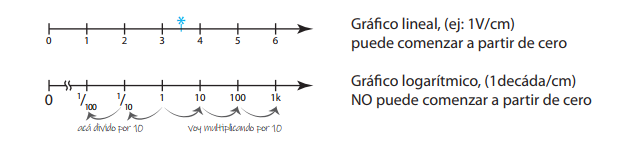
\includegraphics[width=\textwidth]{imagen1}
		\caption{Un gráfico lineal vs. un gráfico logarítmico}
		\centering
	\end{figure}


	\subsection{¿Cuándo usamos una escala logaritmica?}
	La presentación de datos en una escala logarítmica puede ser útil cuando los datos
	cubren una amplia gama de valores - el logaritmo los reduce a un rango más manejable.

	Algunos de nuestros sentidos funcionan de manera logarítmica (ley de Weber-Fechner),
	lo que hace especialmente apropiadas a las escalas logarítmicas para representar 
	estas cantidades. En particular, nuestro sentido del oído percibe cocientes iguales
	de frecuencias como diferencias iguales en el tono.


	\subsection{¿Cómo se hace un gráfico logarítmico?}
	Primero que nada, tenemos que saber que una función $log(x)$ (que es una curva)
	si la trazamos en un gráfico logarítmico se ve como una recta.
	Algo más que tenemos que saber es que la función $log(x)$ no admite $x=0$
	por que la función tiende a $\infty$.

	A continuación podemos ver 3 ejemplos de estos gráficos
	\begin{figure}[H]
		\centering
		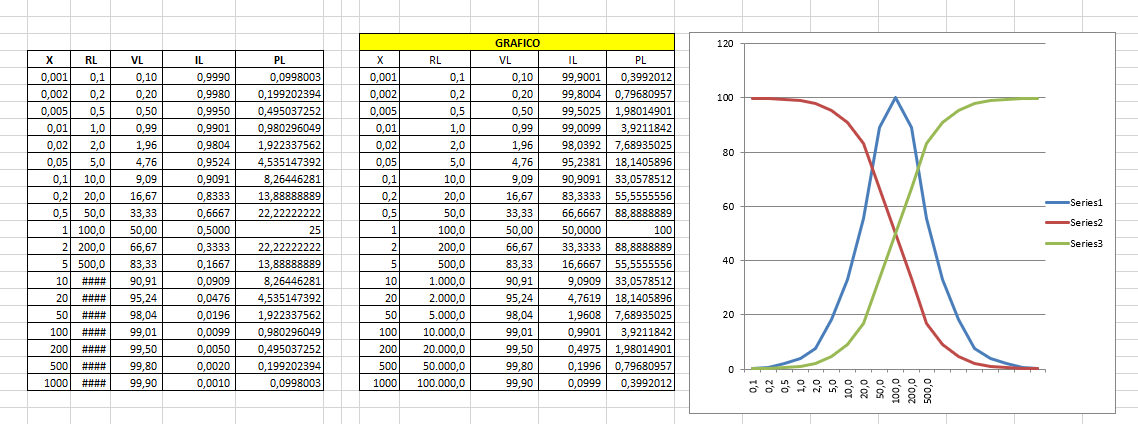
\includegraphics[width=\textwidth]{imagen2.png}
		\caption{Gráfico de la tensión, la corriente y la potencia en función a RL}
		\centering
	\end{figure}


	En este caso vemos como afecta las tensiones, las corrientes, y la potencia
	en función a la RL.\\

	Los valores de RL van a estar en relación a RTH,
	como múltiplos (1x, 2x, 5x, 10x, 20x, etc \ldots{})\\
	o como submúltiplos:(x/2, x/5, x/10, x/20, x/50, x/100, etc \ldots{})

\end{document}
